\documentclass{article}
\usepackage{graphicx}
\usepackage{amsmath}
\usepackage[parfill]{parskip}
\usepackage{hyperref}
\graphicspath{ {./figures/} }

\title{COMP.SEC.220 Security Protocol\footnote{github - \url{https://github.com/ancuongnguyen07/SecurityProtocol}}}
\author{Cuong Nguyen - LAB 1}
\date{29/08/2022}

\begin{document}
    
\maketitle

% EXERCISE 1
\section*{Exercise 1 - Caesar Cipher}
%
\subsection*{Task 1}
%
Keyspace \textbar\ K \textbar\ for the Caesar Cipher is 26 (the number
of characters in English alphabet). So it is possible to do a brute
force attack - 26 keys is super fast to be broken.

\subsection*{Task 2}
%
Because the key space is 26, so any key \(K<0 \ or \ K>25\) is considered
invalid. Mathematically, we could accept key less than 0 or greater 25, but
it makes no sense because it would generate the same result compared to
its correspondant in range 0 to 25:
\begin{align*}
    2 + 12 \equiv 14 \mod 26\\
    2 - 14 \equiv 14 \mod 26\\
    2 + 38 \equiv 14 \mod 26
\end{align*}

% link for referencing https://crypto.stackexchange.com/questions/50645/what-is-wrong-if-you-use-a-key-in-a-caesar-cipher-that-is-greater-than-26

\textbf{Encryption and decrytion time}
\begin{figure}[htp]
    \centering
    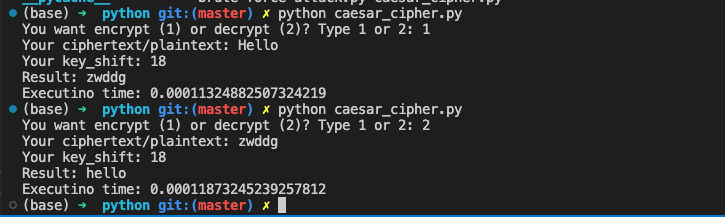
\includegraphics[width=120mm, height=40mm]{caesar_cipher_time.png}
    \caption{Caesar Cipher - Encryption and decrytion time}
    \label{fig:en_de_time}
\end{figure}

\subsection*{Task 3}
The original message is:\\
\textbf{SK COMPLETED. YOU ARE READY FOR THE SECURITY 
PROTOCOLS COURSE- ADMIN}\\ 
Key: 9\\
The program took about \(0.00076\) seconds to break the ciphertext

\begin{figure}[htp]
    \centering
    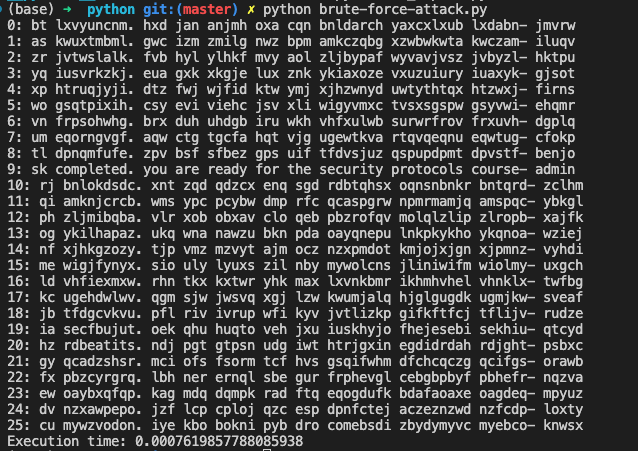
\includegraphics[width=120mm, height=90mm]{brute_force_single_caesar.png}
    \caption{Caesar Cipher - brute force attack time}
    \label{fig:bf_attack_time}
\end{figure}

% EXERCISE 2
\section*{Exercise 2 - Double Caesar Cipher}

The plaintext is:\\
\textbf{WILL TAKE THE RING TO MORDOR, THOUGH I DO NOT KNOW THE WAY}\\
which is used in the movie:
\emph{The Lord of the Rings: The Fellowship of the Rin}

\begin{figure}[htp]
    \centering
    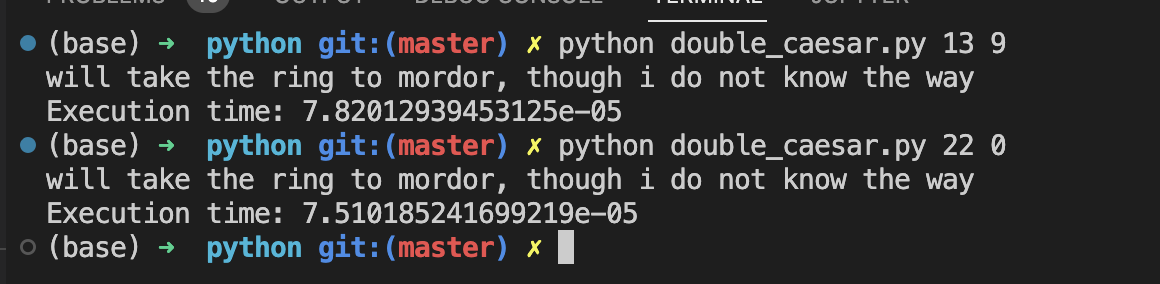
\includegraphics[width=120mm, height=50mm]{double_caesar.png}
    \caption{Double Caesar Cipher decryption time}
    \label{fig:double_caesar_decrypt_time}
\end{figure}

\\
By doubling the encryption, Caesar Cipher isn't more secure because
it works in a group which means that if a message is first encrypted
with a key of 13 then re-encrypted with a key of 9, the result is
equivalent to encrypting the meassage with a key 22 (Figure
~\ref{fig:double_caesar_decrypt_time})

\begin{figure}[htp]
    \centering
    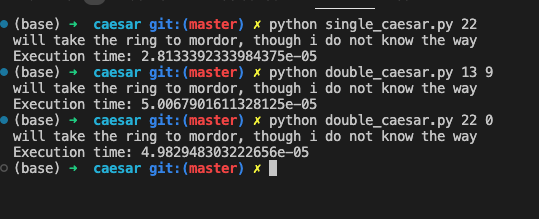
\includegraphics[height=50mm, width=120mm]{single_double_caesar_time.png}
    \caption{Single VS Double Caesar Cipher - execution time}
    \label{fig:single_double_time}
\end{figure}

Compared to original Caesar Cipher, there is a significant performanc
drop off (Figure~\ref{fig:single_double_time})


% EXERCISE 3
\section*{Exercise 3 - Affine Cipher}
Using the keys a = 11, b = 8, the ciphertext of ``securityprotocols'':\\
\textbf{yaeunsjmrngjgegzy}

\begin{figure}[htp]
    \centering
    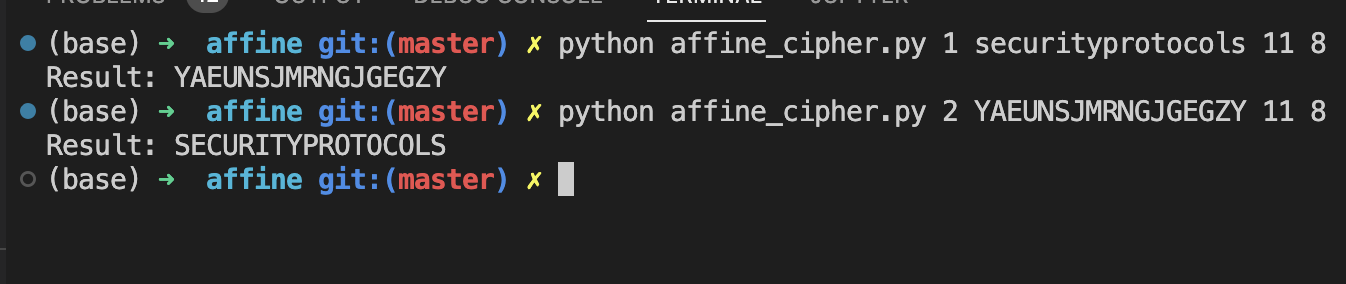
\includegraphics[width=120mm, height=50mm]{affine_encrypt.png}
    \caption{Affine cipher encryption of ``securityprotocols''}
    \label{fig:affine_encrypt}
\end{figure}

Using the keys a = 19, b = 5, the plaintext of ``TLV JIFGG SLC EFJJ'':\\
\textbf{YOU SHALL NOT PASS}

\begin{figure}[htp]
    \centering
    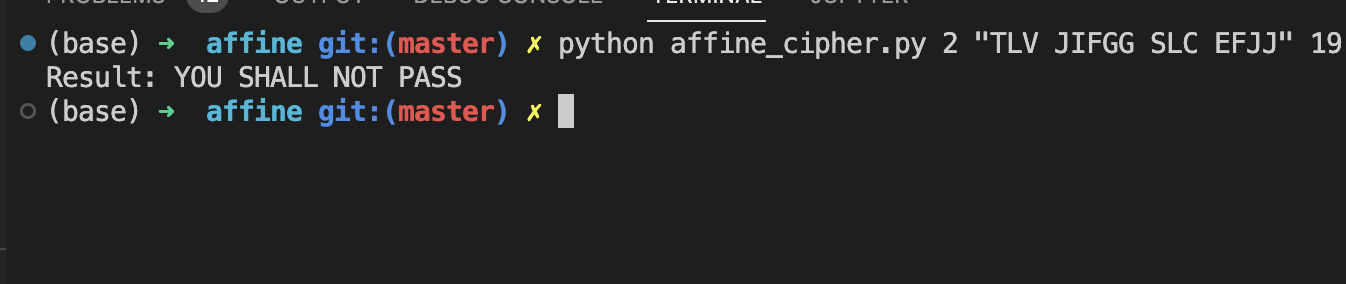
\includegraphics[width=120mm, height=50mm]{affine_decrypt.png}
    \caption{Affine cipher encryption of ``TLV JIFGG SLC EFJJ''}
    \label{fig:affine_decrypt}
\end{figure}

The Caesar cipher is an Affine Cipher with a = 1, they both have a key space
of 26 (the number of characters in English alphabet). So I would say both have
the same level of security.

% EXERCISE 4
\section*{Exercise 4 - Frequency Analysis}
The plaintext is:\\
\textbf{EVEN DARKNESS MUST PASS. A NEW DAY WILL COME. AND WHEN THE SUN SHINES 
IT WILL SHINE OUT THE CLEARER. THOSE WERE THE STORIES THAT STAYED WITH YOU,
THAT MEANT SOMETHING, EVEN IF YOU WERE TOO SMALL TO UNDERSTAND WHY." IN WHICH
MOVIE WAS THIS QUOTE SAID, WHO SAID IT AND TO WHOM WAS HE SPEAKING TO? HINT:
THE BEST FANTASY MOVIE TRILOGY OF ALL TIME}\\
\(\rightarrow\ \)The answer is \emph{The Dark Knight}

\begin{figure}[htp]
    \centering
    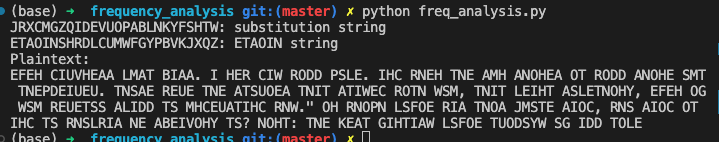
\includegraphics[width=120mm, height=50mm]{naive_freq_analysis.png}
    \caption{Naive Frequency Analysis}
    \label{fig:naive_freq_analysis}
\end{figure}

\begin{figure}[htp]
    \centering
    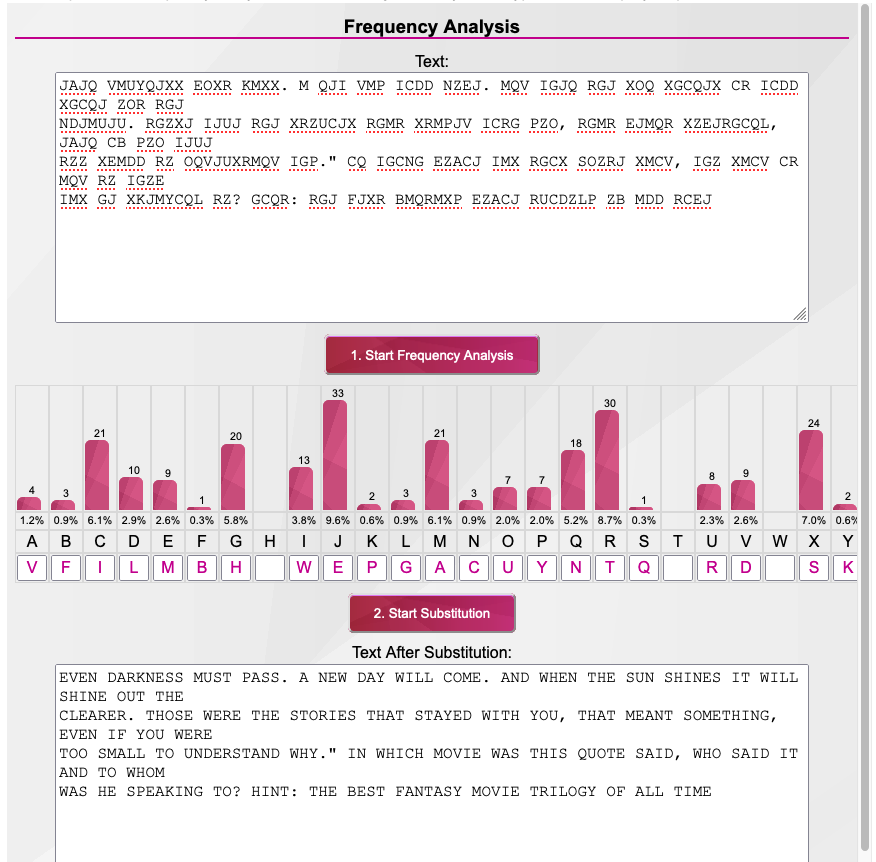
\includegraphics[width=120mm, height=120mm]{modified_freq_analysis.png}
    \caption{Manually Modified Frequency Analysis}
    \label{fig:modified_freq_analysis}
\end{figure}

The most common letter in the cipher is ``J'' which is different from the most
common letter in the english language ``E''

The least common letters in the cipher is ``F,S'' which are different from the
least commont letters in the english language ``J,Q,Z''

It took me about half an hour to crack the cipher, so I think this approach isn't
secure enough. Remember that the longer the ciphertext is the easier it might be
broken, because the frequency statistics would fit the \emph{the most common English
letter, ETAOIN}, very well. 
\end{document}